\documentclass[11pt]{article}
\usepackage{hyperref}
\usepackage{graphicx}
\title{\textbf{Mobile Middleware Project: Sauna-App}}
\author{Leo Muona \and
		Eeva Terkki}
\date{\today}
\begin{document}

\maketitle
\thispagestyle{empty}

\section{Description}

Sauna-App is an Android application for enhancing the user's sauna experience with the help of SensorDrone\footnote{http://sensorcon.com/sensordrone/}. It supports Android 2.2 and newer versions. When the sensor is placed in the sauna, the application can be used, for example, to check the temperature from another room while waiting for the sauna to heat up, or to ensure that the carbon monoxide concentration is at a safe level. In order for user to start using the software, SensorDrone's MAC address must be specified in the application's settings. The current version of Sauna-App provides the following functionality:\\

\noindent\textbf{Measuring and displaying sensor data:} When the \textit{Measure} button on the main view is clicked, SensorDrone measures the temperature, humidity, and carbon monoxide concentration of the sauna. The results are displayed on the screen. \\

\noindent\textbf{User preferences:} In the application menu, the user can choose to change the default user preferences. Currently, the available values are favorite temperature and humidity. After measuring, the application informs how well these preferences are met. \\

\noindent\textbf{CO warnings:} After measuring, the application gives an alert if the carbon monoxide concentration in the sauna is high. A warning about a harmful CO level is given when the concentration is 35.0 ppm or more, and the value is displayed in yellow. When the concentration is 100.0 ppm or more, a warning about a high CO level is given and the value is displayed in red\footnote{The source for the limits is \url{http://en.wikipedia.org/wiki/Carbon_monoxide_poisoning\#Signs_and_symptoms}. The application cannot replace a real carbon monoxide detector.}.

\section{Possible Future Improvements}

As of now, the application is quite basic. However, future improvements have been thought of in order to enhance user experience and make the application more smart. \\

\noindent\textbf{Warming up state:} A simple improvement to the application would a "warming up state". In this state the application would measure sauna state for example every five minutes and when the sauna temperature would rise to be within user's preferenced temperature, it would notify it to the user. This way, user wouldn't have to measure the temperature manually every time to check if the sauna is warm enough via \textit{Measure} button. \\

\noindent\textbf{Cloud functionalities:} No server-side functionality is currently available, but the next implementation step would be to upload the collected sensor data to the cloud. The data related to a user profile could be used for publishing statistics of e.g. the average length and temperature of their sauna visits. The server could also analyze data collected from several users, for example to create default user preference profiles based on age and gender. \\

\noindent\textbf{Smarter user profiles:} In the future, the application could be made smarter so that instead of the user adjusting the preferred temperature and humidity values in their profile, the server would try to find the optimal values for each user based on their earlier sauna sessions. The user could rate each sauna session and the feedback would be linked to the sensor data obtained during the session. The results would then be compared with previously collected data and the user's preferences would be adjusted if necessary. To implement this, measuring should be done periodically without the user having to press the \textit{Measure} button. Another enhancement to user profiles would be to have different profiles for different sauna types. For example, if user would like to use the application with turkish saunas and finnish saunas, there should be different measurement profiles for those. \\

\noindent\textbf{Friends and sauna invites:} Another new feature to the application could be a "friend functionality", where the user can add other Sauna-App users as friends. The application could be configured to automatically send a message to selected friends when the sauna is ready, inviting them over. \\

\section{Architecture}
\begin{figure}[h!]
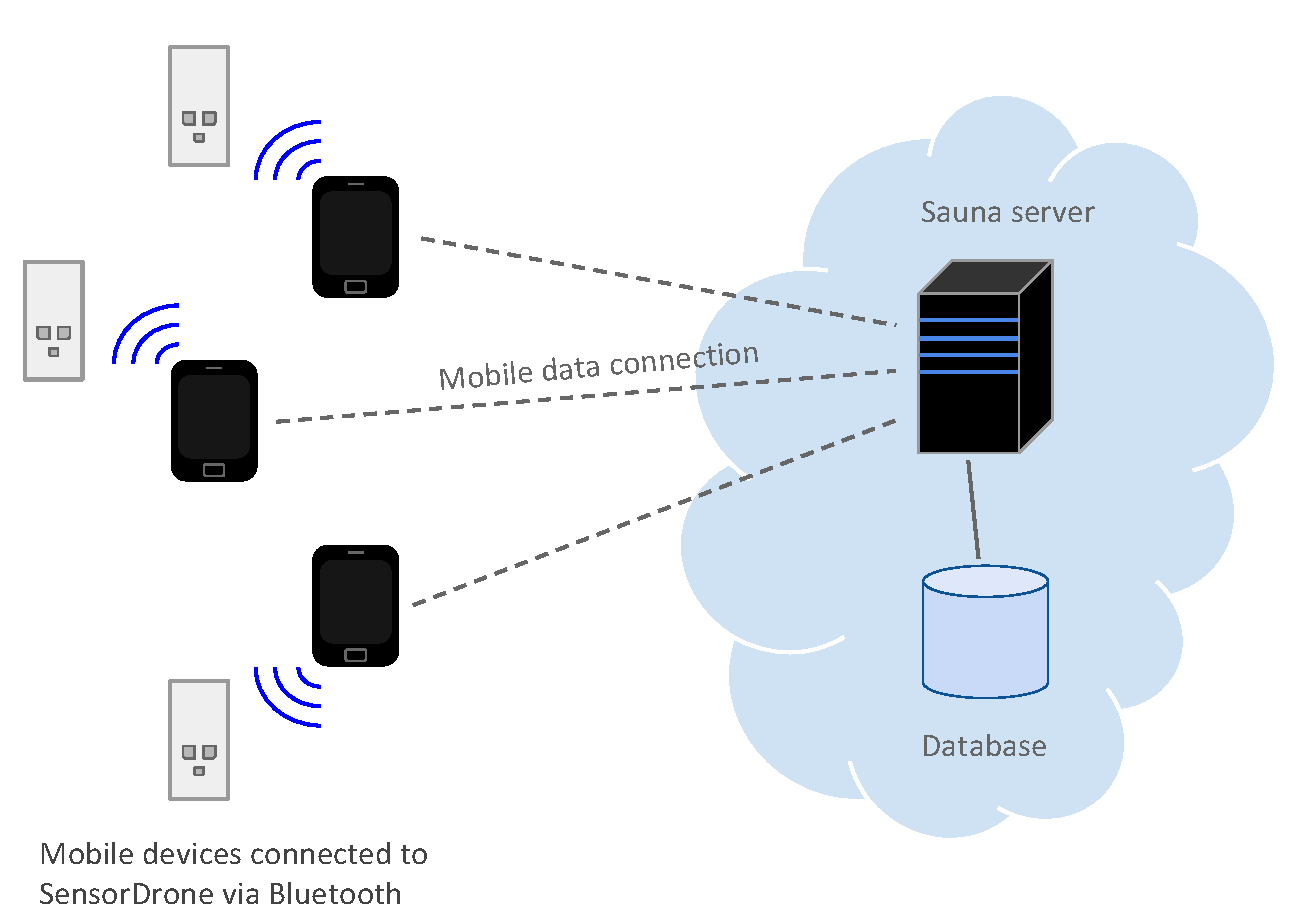
\includegraphics[width=\textwidth, height=\textheight, keepaspectratio]{design.pdf}
\end{figure}

\end{document}
